% Presentación del Taller 1 · NovaRetail 360.  Compilar:  make presentacion  (ver ../Makefile)
\documentclass[aspectratio=169,10pt]{beamer}
\usepackage[spanish,es-noshorthands]{babel}
\usetheme{UD}

\newcommand{\kpi}[3]{% valor, etiqueta, color
  \UDCard{white}{UDBorder}{{\cambriafont\fontsize{17pt}{19pt}\selectfont\bfseries\color{#3}#1}\par{\fontsize{7.5pt}{9pt}\selectfont #2}}}
\newcommand{\peq}{\fontsize{8pt}{9.6pt}\selectfont}

\begin{document}

\UDportada{NovaRetail 360}
          {Power Query, modelo relacional y SQL}
          {Juan Felipe Rodríguez Galindo\\{\fontsize{6.4pt}{7.4pt}\selectfont\mdseries\color{UDSilver}20261595004}}
          {Maestría en Ciencias de la Información y las Comunicaciones}
          {Inteligencia de Negocios · 2026}

% ---------------------------------------------------------------- 2
\begin{frame}{El reto y los datos}{La gerencia no puede usar los datos tal como llegan}
  \begin{columns}[T,onlytextwidth]
    \begin{column}{0.48\textwidth}
      \UDCard{white}{UDBorder}{\cardtitle{UDBlue}{Qué necesita la gerencia}{\peq
        Ventas netas, devoluciones, mezcla de canales, cumplimiento de metas y comportamiento regional (enero--junio 2026).}}
      \vspace{0.2cm}
      \UDCard{UDLightGray}{UDRed!60}{\cardtitle{UDRed}{Qué se recibió}{\peq
        5 CSV con datos sintéticos e incidencias intencionales. Las 13 incidencias están todas en \texttt{ventas}.}}
    \end{column}
    \begin{column}{0.48\textwidth}
      \begin{tabular}{@{}lr@{}}
        \peq ventas\_sucias & \peq 1\,201 \\
        \peq clientes & \peq 120 \\
        \peq productos & \peq 40 \\
        \peq devoluciones & \peq 70 \\
        \peq metas (6 meses $\times$ 5 regiones) & \peq 30 \\
      \end{tabular}
      \vspace{0.25cm}

      {\peq\color{UDSilver} Se entrega pipeline Python/SQLite verificado y \texttt{NovaRetail360.pbix}: las consultas M se ejecutaron en Power BI y cuadran con el pipeline.}
    \end{column}
  \end{columns}
  \note{Contar que al ejecutar las consultas en Power BI apareció la fecha inexistente 2026-02-30 (V00312), que el pipeline aceptaba; se corrigió y las cifras ya la incluyen.}
\end{frame}

% ---------------------------------------------------------------- 3
\begin{frame}{Parte A · Doce incidencias, cada una con su regla}{Se corrigen 5, se auditan 7 y no se borra nada en silencio}
  \begin{columns}[T,onlytextwidth]
    \begin{column}{0.48\textwidth}
      \UDCard{white}{UDGreen!60}{\cardtitle{UDDarkGreen}{Corregidas (5)}{\peq
        \textbf{Fecha} \texttt{15/02/2026} $\to$ ISO (día $>$12)\\
        \textbf{Canal} \texttt{web\textvisiblespace}, \texttt{WEB} $\to$ Web\\
        \textbf{Precio} vacío o $-20\,000$ $\to$ precio de lista (1\,198/1\,198 ventas válidas lo cumplen)}}
    \end{column}
    \begin{column}{0.48\textwidth}
      \UDCard{UDLightGray}{UDRed!60}{\cardtitle{UDRed}{A auditoría (7)}{\peq
        Venta repetida (V00240)\\
        Fecha vacía (V00039)\\
        Cliente \texttt{C9999} y producto \texttt{P999} inexistentes\\
        Cantidad $-2$ y vacía\\
        Descuento del 125\,\%}}
    \end{column}
  \end{columns}
  \vspace{0.3cm}
  \begin{center}
  \begin{tikzpicture}[node distance=0.35cm]
    \node[paso] (a) {\textbf{1\,201}\\crudas};
    \node[paso, right=of a, fill=UDGreen!8, draw=UDGreen] (b) {\textbf{1\,193}\\aceptadas};
    \node[paso, right=of b, fill=UDRed!8, draw=UDRed] (c) {\textbf{8}\\auditoría};
    \node[right=0.35cm of c, text width=3.4cm, font=\fontsize{7.5pt}{9pt}\selectfont] {1\,193 + 8 = 1\,201: el cuadre se verifica en el código.};
    \draw[flecha] (a) -- (b); \draw[flecha] (b) -- (c);
  \end{tikzpicture}
  \end{center}
\end{frame}

% ---------------------------------------------------------------- 4
\begin{frame}{El total engaña, la composición no}{Conciliación entre la suma ingenua del archivo y el conjunto depurado}
  \begin{columns}[T,onlytextwidth]
    \begin{column}{0.55\textwidth}
      {\peq
      \begin{tabular}{@{}lr@{}}
        Suma ingenua del archivo & 701\,679\,450 \\
        Venta repetida & $-1\,015\,920$ \\
        Cliente y producto inexistentes & $-2\,024\,160$ \\
        Fecha vacía o inexistente & $-793\,510$ \\
        Cantidad $-2$ y descuento 125\,\% & $+551\,800$ \\
        Precios imputados & $+978\,000$ \\
        \midrule
        \textbf{Depurado} & \textbf{699\,375\,660} \\
      \end{tabular}}
    \end{column}
    \begin{column}{0.4\textwidth}
      \kpi{0,33\,\%}{diferencia entre ambos totales}{UDRed}
      \vspace{0.2cm}

      {\peq Unos errores suman y otros restan: el total ``parece bien'' aunque la composición por región, canal o mes sea errónea.}
    \end{column}
  \end{columns}
\end{frame}

% ---------------------------------------------------------------- 5
\begin{frame}{Reproducibilidad y riesgos}{Pasos aplicados de Power Query frente a reemplazos sin regla}
  \begin{columns}[T,onlytextwidth]
    \begin{column}{0.48\textwidth}
      \UDCard{white}{UDBlue!60}{\cardtitle{UDBlue}{Lo que sí repite el proceso}{\peq
        Cada transformación queda como línea M en \emph{Applied Steps}. Un archivo nuevo repite los mismos pasos, en el mismo orden, y la receta se puede leer y versionar.}}
    \end{column}
    \begin{column}{0.48\textwidth}
      \UDCard{UDLightGray}{UDRed!60}{\cardtitle{UDRed}{Riesgos de reemplazar valores}{\peq
        Sesgo silencioso (vacío $\to$ 0)\\
        Se pierde el valor original\\
        El literal no sirve en la próxima entrega\\
        Dependencia del orden de los pasos}}
    \end{column}
  \end{columns}
  \vspace{0.3cm}
  {\peq Lo adoptado: reglas como \textbf{condiciones} (no valores), registro original conservado y una consulta de auditoría complementaria.}
\end{frame}

% ---------------------------------------------------------------- 6
\begin{frame}{Parte B · Modelo operacional}{Cinco tablas, un hecho y cardinalidades explícitas}
  \begin{center}
  \begin{tikzpicture}[
    ent/.style={draw=UDBorder, fill=white, rounded corners=2pt, align=left, font=\fontsize{7pt}{8.4pt}\selectfont, inner sep=3pt, text width=2.3cm},
    lin/.style={thick, UDSable!70}, car/.style={font=\fontsize{7pt}{8pt}\selectfont\bfseries, color=UDRed}]
    \node[ent] (c) at (0,0) {\textbf{clientes}\\PK id\_cliente\\region, segmento};
    \node[ent] (p) at (7.8,0) {\textbf{productos}\\PK id\_producto\\categoria, precio\_lista};
    \node[ent, fill=UDRed!8, draw=UDRed] (v) at (3.9,-1.6) {\textbf{ventas}\\PK id\_venta\\FK id\_cliente, id\_producto\\fecha, canal, cantidad, precio, descuento};
    \node[ent] (d) at (3.9,-3.9) {\textbf{devoluciones}\\PK id\_devolucion\\FK id\_venta, cantidad\_devuelta};
    \node[ent] (m) at (0,-3.2) {\textbf{metas}\\PK (periodo, region)\\meta\_ventas};
    \draw[lin] (c) -- node[car, above, pos=.3]{1} node[car, above, pos=.8]{N} (v);
    \draw[lin] (p) -- node[car, above, pos=.3]{1} node[car, above, pos=.8]{N} (v);
    \draw[lin] (v) -- node[car, right, pos=.25]{1} node[car, right, pos=.8]{0..N} (d);
    \draw[lin, dashed] (c) -- (m);
    \node[font=\fontsize{6.5pt}{8pt}\selectfont\itshape, anchor=west] at (0.15,-1.9) {lógica, por región};
  \end{tikzpicture}
  \end{center}
\end{frame}

% ---------------------------------------------------------------- 7
\begin{frame}{Granularidad: por qué no unir metas a cada venta}{Fan-out medido en la base}
  \begin{columns}[T,onlytextwidth]
    \begin{column}{0.3\textwidth}
      \kpi{1\,193}{filas de ventas: una por transacción}{UDBlue}
      \vspace{0.15cm}
      \kpi{30}{filas de metas: una por mes y región}{UDBlue}
    \end{column}
    \begin{column}{0.66\textwidth}
      {\peq Unir \texttt{metas} a cada venta repite la meta de su mes y región unas 40 veces.}
      \vspace{0.15cm}

      \UDCard{UDLightGray}{UDRed!60}{\cardtitle{UDRed}{Efecto sobre la suma de metas}{\peq
        Correcta: \$\,1\,715 millones\\
        Con el JOIN directo: \$\,68\,322 millones (\textbf{39,8 veces})}}
      \vspace{0.15cm}

      {\peq Regla: agregar ventas a (mes, región) \textbf{antes} de unir.}
    \end{column}
  \end{columns}
\end{frame}

% ---------------------------------------------------------------- 8
\begin{frame}{Operacional frente a estrella}{La estrella está implementada y concilia con diferencia 0}
  {\fontsize{7.8pt}{9.4pt}\selectfont
  \begin{tabular}{@{}p{1.7cm}p{4.5cm}p{4.5cm}@{}}
    \toprule
     & \textbf{Operacional normalizado} & \textbf{Esquema estrella} \\
    \midrule
    Objetivo & Capturar transacciones sin redundancia & Responder preguntas analíticas con pocas uniones \\[2pt]
    Estructura & 5 tablas en 3FN, uniones por FK & 3 hechos (ventas, devoluciones, metas) y 4 dimensiones (fecha, cliente, producto, canal) \\[2pt]
    Metas & Se unen con cuidado (distinto grano) & Hecho propio mes--región, dimensiones conformadas \\[2pt]
    Riesgo & Fan-out por olvidar el grano & Dimensiones mal conformadas \\
    \bottomrule
  \end{tabular}}
\end{frame}

% ---------------------------------------------------------------- 9
\begin{frame}{Parte C · SQL que audita}{LEFT JOIN muestra el problema; INNER JOIN lo esconde}
  \begin{columns}[T,onlytextwidth]
    \begin{column}{0.48\textwidth}
      \UDCard{white}{UDBlue!60}{\cardtitle{UDBlue}{INNER frente a LEFT}{\peq
        Datos crudos: 1\,201 filas.\\
        \texttt{INNER JOIN} devuelve 1\,199; las 2 huérfanas desaparecen sin aviso.\\
        \texttt{LEFT JOIN ... IS NULL} las lista: V00054 y V00073.}}
    \end{column}
    \begin{column}{0.48\textwidth}
      \UDCard{white}{UDBorder}{\cardtitle{UDSable}{Conceptos}{\peq
        \texttt{WHERE} filtra filas antes de agrupar; \texttt{HAVING}, grupos ya agregados.\\
        \texttt{COUNT(*)} = 1\,201; \texttt{COUNT(DISTINCT id\_venta)} = 1\,200: la diferencia es el duplicado V00240.}}
    \end{column}
  \end{columns}
  \vspace{0.2cm}
  {\peq Verificación cruzada con \texttt{consultas\_referencia.sql}: Q1 y Q5 coinciden fila a fila; Q2 y Q4 dan los mismos valores.}
\end{frame}

% ---------------------------------------------------------------- 10
\begin{frame}{Resultado 1 · Ninguna meta se cumple}{Cumplimiento = ventas netas / meta, por mes y región}
  \begin{columns}[T,onlytextwidth]
    \begin{column}{0.64\textwidth}
      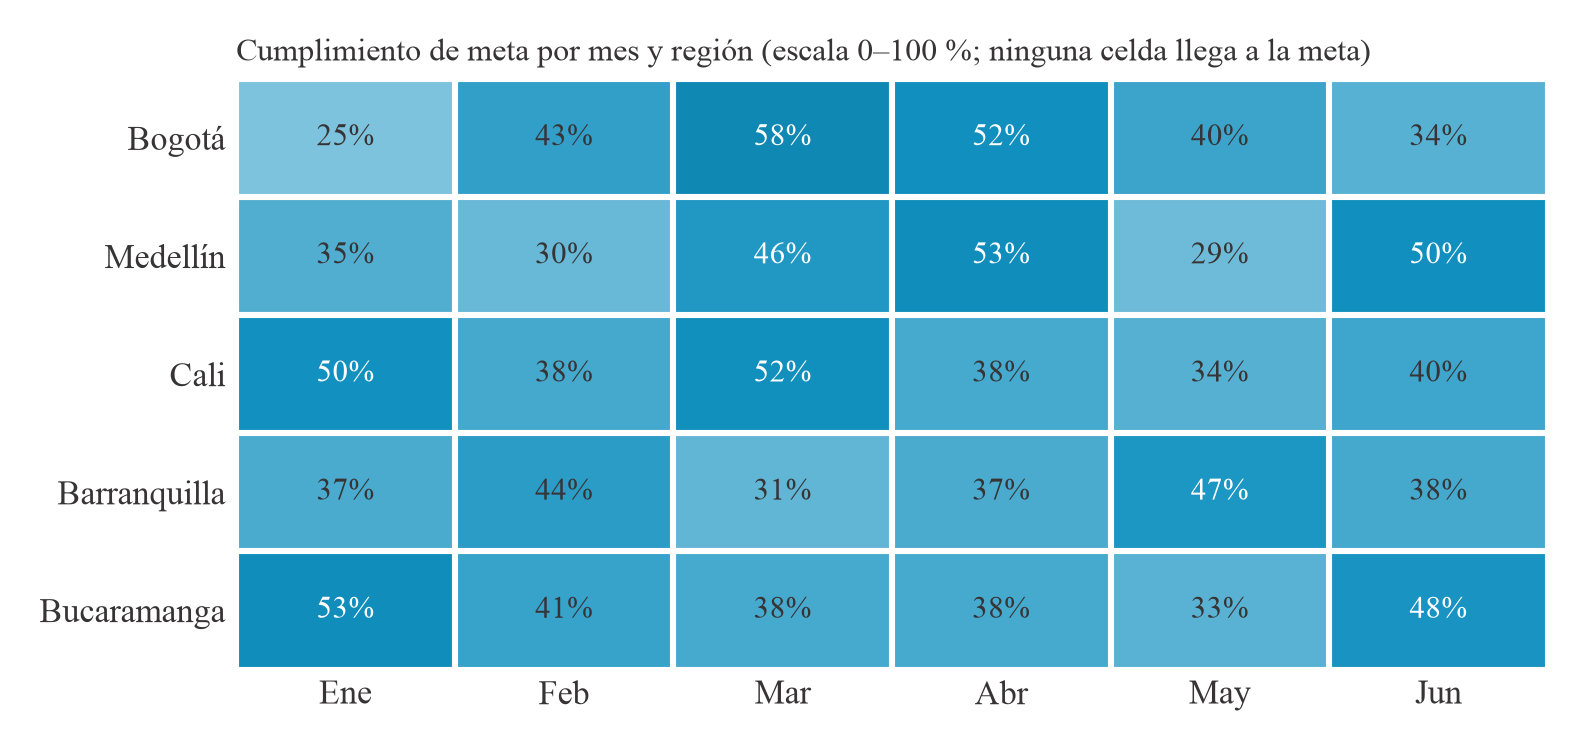
\includegraphics[width=\linewidth]{../salida/figuras/cumplimiento_heatmap.png}
    \end{column}
    \begin{column}{0.32\textwidth}
      \kpi{40,8\,\%}{cumplimiento global (699,4 de 1\,715 millones)}{UDRed}
      \vspace{0.12cm}

      {\peq 0 de 30 combinaciones cumplen. Entre regiones la diferencia es mínima: 38,7\,\% a 41,8\,\%.}
    \end{column}
  \end{columns}
\end{frame}

% ---------------------------------------------------------------- 11
\begin{frame}{Resultado 2 · Devoluciones y canales}{Tecnología concentra las devoluciones; los canales pesan igual}
  \begin{columns}[T,onlytextwidth]
    \begin{column}{0.58\textwidth}
      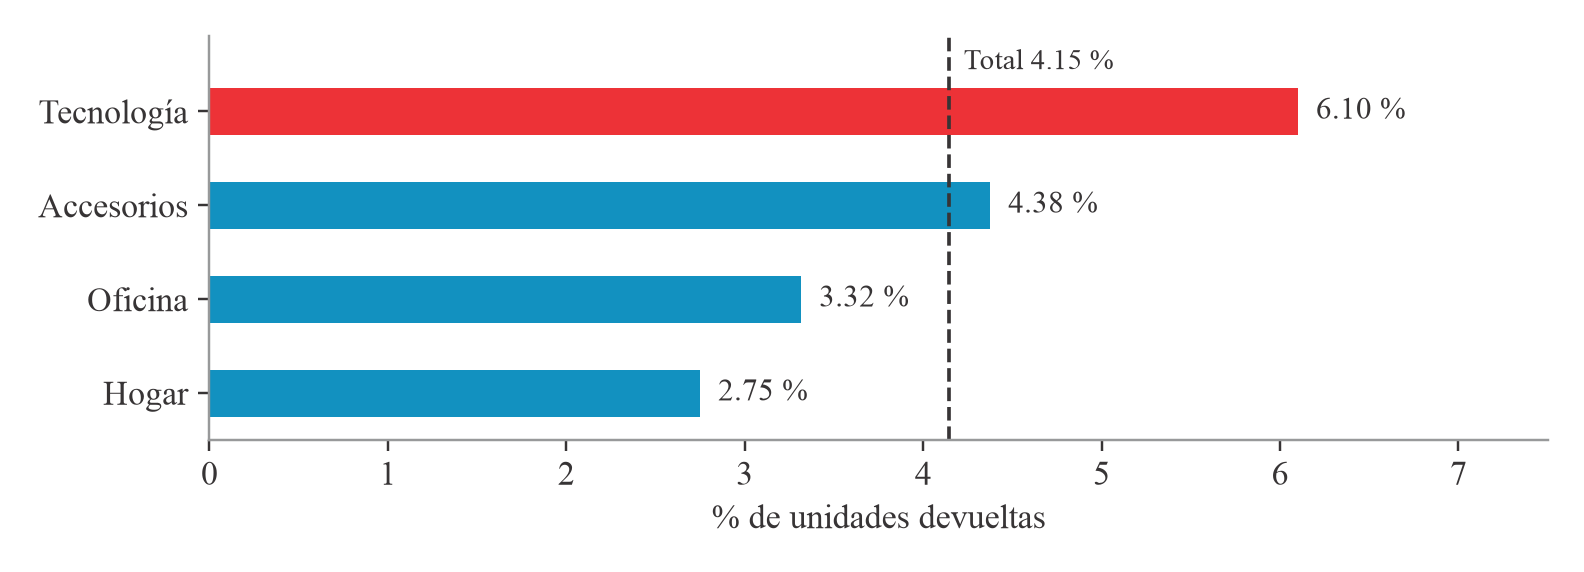
\includegraphics[width=\linewidth]{../salida/figuras/devolucion_categoria.png}
      \vspace{0.1cm}

      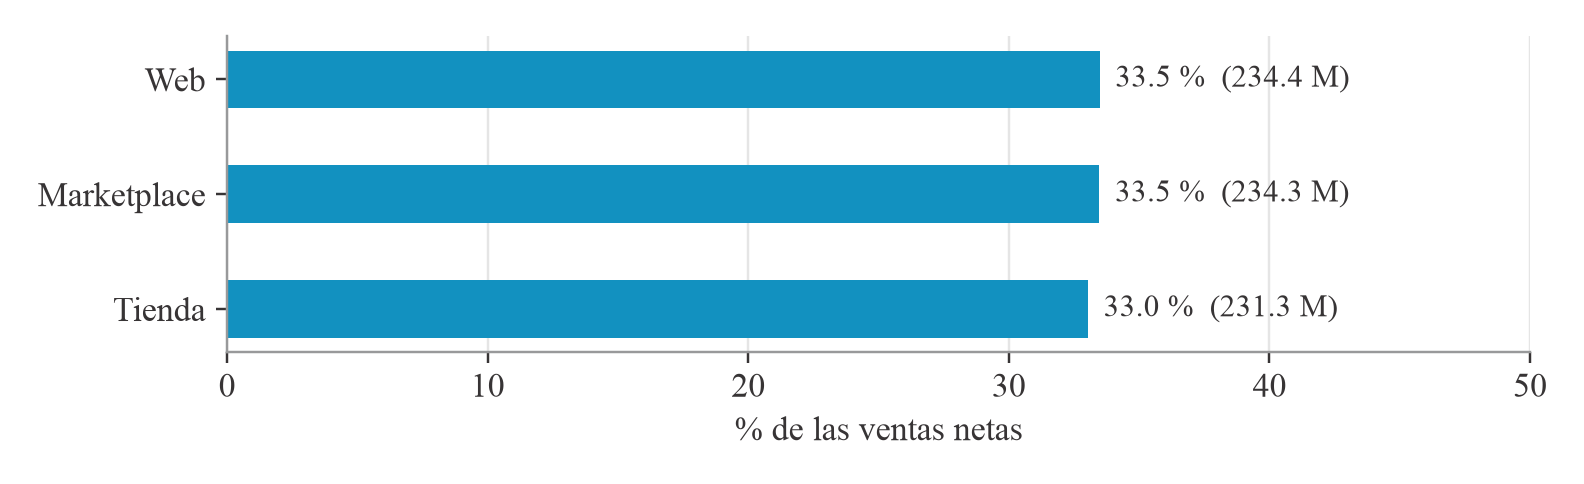
\includegraphics[width=\linewidth]{../salida/figuras/canal.png}
    \end{column}
    \begin{column}{0.38\textwidth}
      \kpi{4,15\,\%}{de unidades devueltas (4,28\,\% del valor)}{UDBlue}
      \vspace{0.12cm}

      {\peq Tecnología 6,10\,\% frente a Hogar 2,75\,\%. Web, Marketplace y Tienda: 33,5\,\% / 33,5\,\% / 33,0\,\%.}
    \end{column}
  \end{columns}
\end{frame}

% ---------------------------------------------------------------- 12
\begin{frame}{Recomendación ejecutiva}{Con sus límites a la vista}
  \begin{columns}[T,onlytextwidth]
    \begin{column}{0.48\textwidth}
      \UDCard{white}{UDRed!60}{\cardtitle{UDRed}{Qué hacer}{\peq
        \textbf{1.} Validar cómo se definió la meta antes de juzgar regiones: una brecha tan pareja sugiere meta mal escalada.\\
        \textbf{2.} Investigar Tecnología (defecto o cambio, proveedor).\\
        \textbf{3.} Mantener los tres canales; el canal no discrimina.}}
    \end{column}
    \begin{column}{0.48\textwidth}
      \UDCard{UDLightGray}{UDBorder}{\cardtitle{UDSilver}{Limitaciones}{\peq
        Datos sintéticos y 6 meses.\\
        Sin costos: ingreso, no margen.\\
        8 registros rechazados y 2 precios imputados: confirmar con el dueño del dato.\\
        Validado en Power BI (\texttt{NovaRetail360.pbix}).}}
    \end{column}
  \end{columns}
\end{frame}

\UDcierre{Juan Felipe Rodríguez Galindo}
         {Maestría en Ciencias de la Información\\y las Comunicaciones}
         {Inteligencia de Negocios · Taller 1}

\end{document}
